\documentclass[xcolor=pdftex,x11names,table,hyperref]{beamer}

\usepackage{verbatim}
\usepackage{setspace}
\usepackage{url}
\usepackage{xcolor} % See documentation PDF at http://www.ctan.org/pkg/xcolor
\definecolor{darkgreen}{rgb}{0,0.3,0}
\definecolor{darkblue}{rgb}{.05,.05,.30}
\definecolor{lightgrey}{rgb}{0.65,0.65,0.65}
\usepackage{tikzsymbols}


\setbeamertemplate{section in toc}[sections numbered]
\setbeamertemplate{subsection in toc}[subsections numbered]
\setbeamertemplate{subsubsection in toc}[subsubsections numbered]
\usetheme{Singapore}
\setbeamertemplate{navigation symbols}{}
\setbeamertemplate{footline}{%
\vspace{0.0em}%
\hspace{0.5em}%
{\color[rgb]{.1,.1,.1} \insertframenumber{}~/~\inserttotalframenumber}
}

\newcommand{\code}[1]{{\color{darkgreen}\texttt{#1}}}
\newcommand{\detail}[1]{{\color{lightgrey}\small{}#1}}
\newcommand{\teeny}[1]{\scalebox{0.09}{#1}}
\newcommand{\tablecolors}{\rowcolors{2}{blue!12}{white}} % Cool table colors


\begin{document}

\title{\LARGE{Words} \\[1.0em] \small{and their abstractions} \\[1.5em]
 %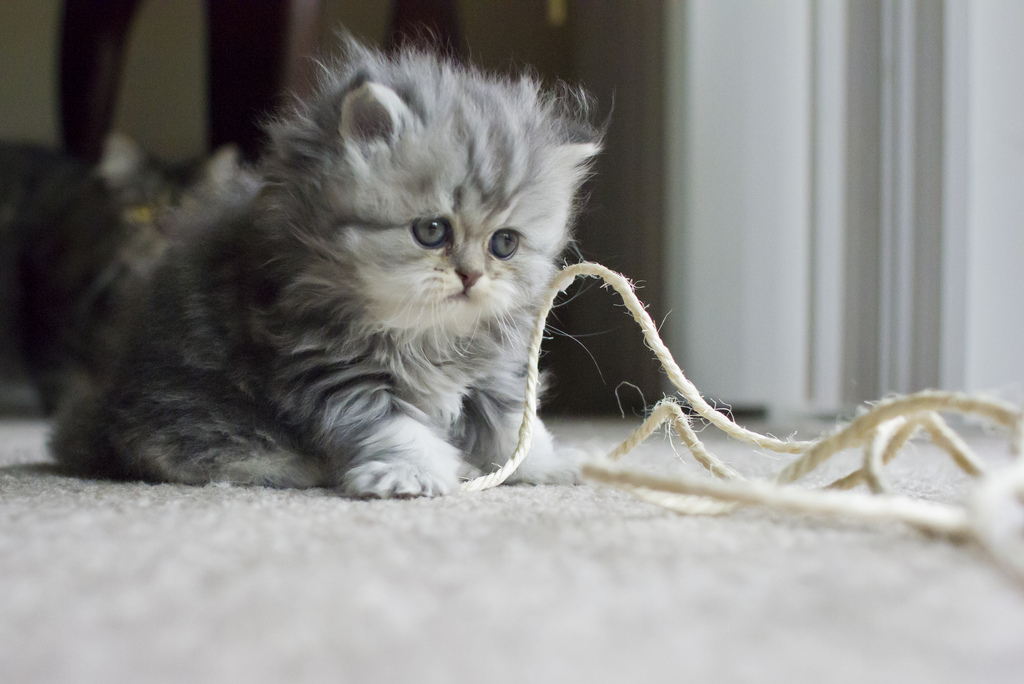
\includegraphics[width=0.5\textwidth]{images/kitten_string_flickr_albaraa.jpg} \\[-1.0em]
 %\small{Possibilities} \\[1.0em]
 %LT1 \\[1.0em]
 }
\author{\href{http://jon.dehdari.org}{Jon Dehdari}}
\frame{\titlepage}

% examples: days of week, company names, first/last names
\begin{frame}{Too Many Words!}
	{\center 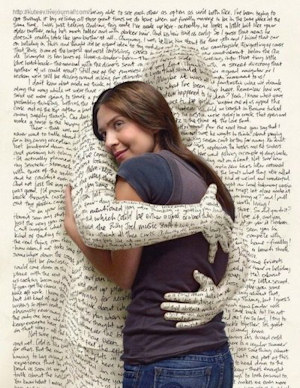
\includegraphics[width=0.33\textheight]{images/word-lover.jpg}}
\begin{itemize}
	\item Languages have too many words for statistical models of language
	\pause
	\item We need some way to generalize them
	\pause
	\item Let's treat some words like other words
\end{itemize}
\end{frame}

\begin{frame}{}
\begin{itemize}
	\item Words can be grouped together into equivalence classes to help reduce data sparsity and better generalize the data.

\begin{center}
	\pause
	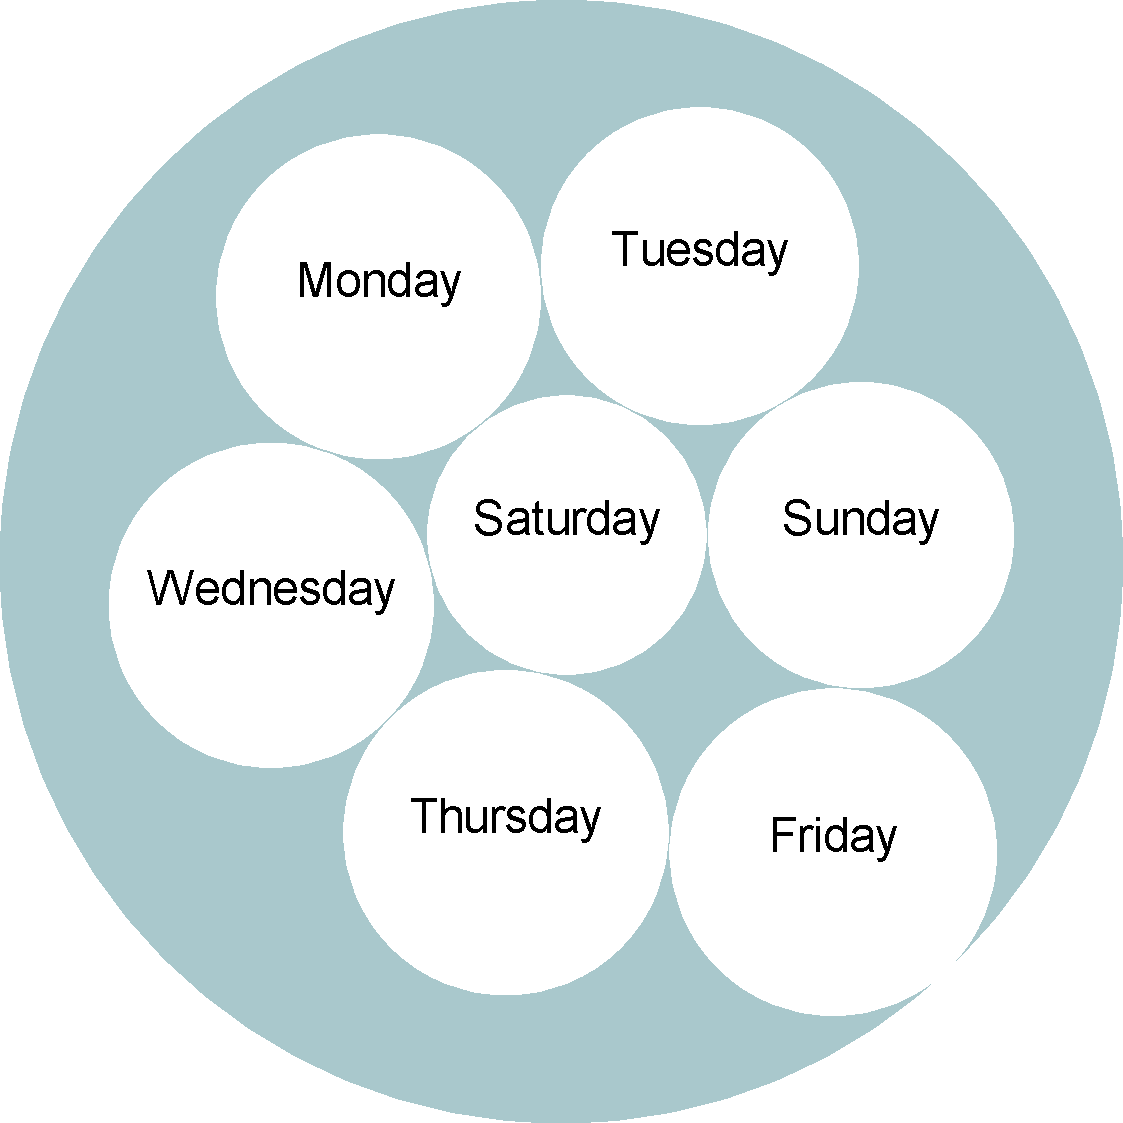
\includegraphics[width=0.45\textheight]{images/clusters_days.pdf}
	\hspace*{1.3em}%
	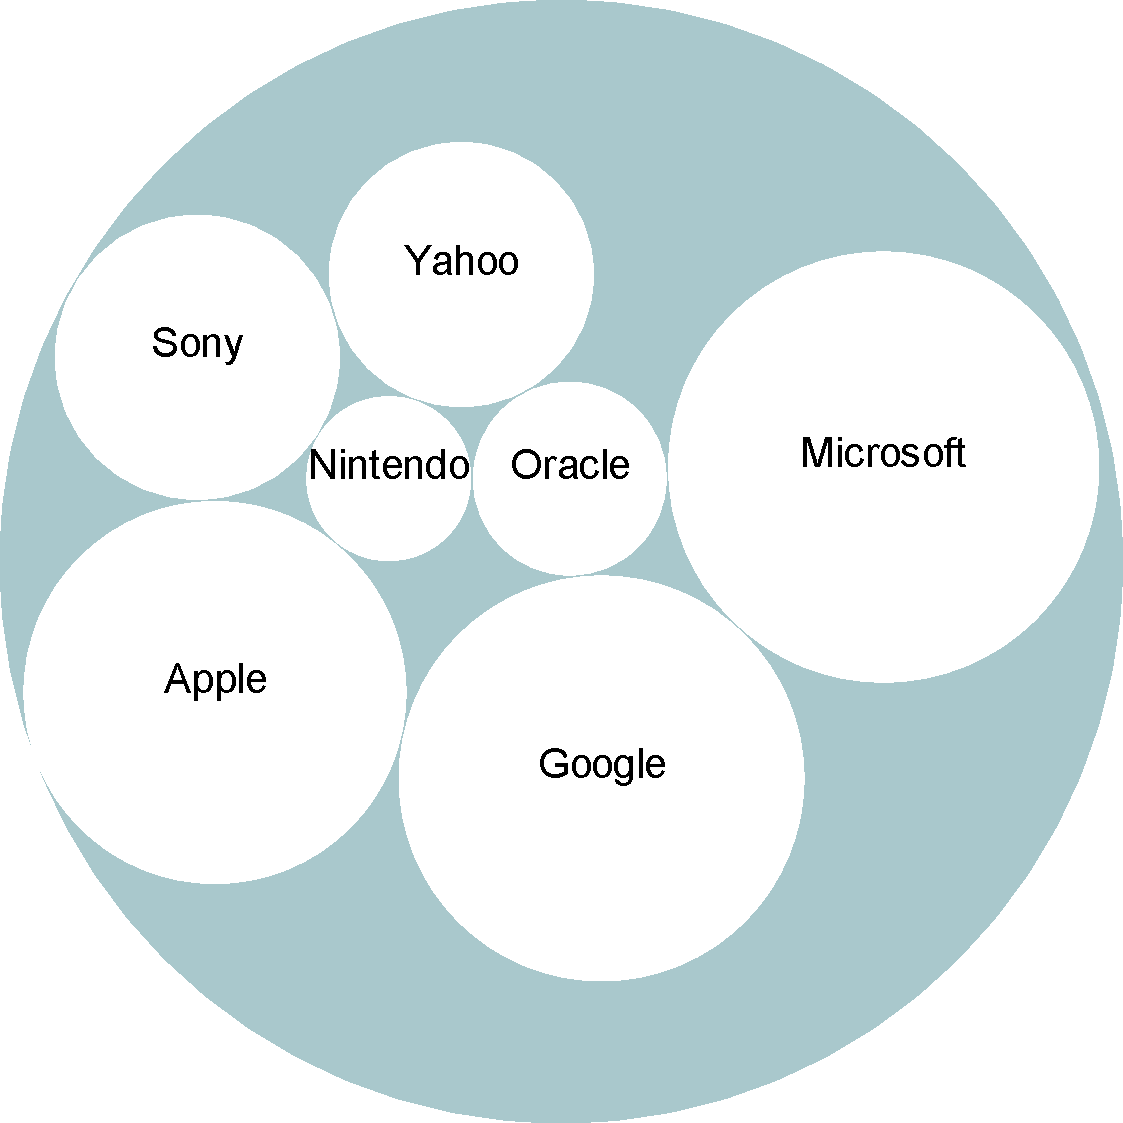
\includegraphics[width=0.45\textheight]{images/clusters_tech_companies.pdf}%
\end{center}
\pause

	\item Hand-crafted equivalence classes are called \textbf{part-of-speech tags}, and automatically induced equivalence classes are usually called \textbf{word classes} or \textbf{word clusters}
\end{itemize}
\end{frame}

% parts of speech
\begin{frame}{Parts of Speech and Word Clusters}
\begin{itemize}
	\item Part-of-speech example: \\[0.7em]
		\begin{scriptsize}
		\begin{tabular}{lllllllllll}
			Pierre & Vinken & , & 61 & years & old & , & will & join & the & board \\
			NNP & NNP & , & CD & NNS & JJ & , & MD & VB & DT & NN \\
		\end{tabular}
	\end{scriptsize} \\[1.0em]

	\item Word cluster example: \\[0.7em]
		\begin{scriptsize}
		\begin{tabular}{lllllllllll}
			Pierre & Vinken & , & 61 & years & old & , & will & join & the & board \\
			344 & 0 & 283 & 94 & 348 & 274 & 283 & 367 & 360 & 71 & 390 \\[0.8em]
		\end{tabular}
		\end{scriptsize}
	\pause
	\hspace*{-1.5em}\textbf{Differences}:
	\item Parts of speech have human-readable labels (eg.\ NN, VB), while word clusters usually just have numbers
	\item A word can have more than one part of speech (which depends on the context), while a word usually has just one word class
\end{itemize}
\end{frame}

\begin{frame}{Supervised, Unsupervised, Semi-supervised Learning}
\begin{itemize}
	\item \small{\textbf{Supervised learning} uses \textbf{manually-annotated data}} \hfill
		\raisebox{-2.0em}{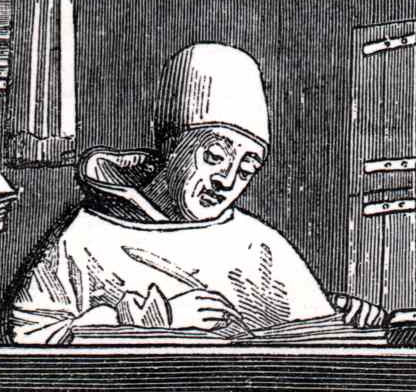
\includegraphics[width=0.13\textwidth]{images/scriptorium-monk-at-work-crop.jpg}}
	\begin{itemize}
		\pause
		\item It's usually expensive and small
		\pause
		\item It's usually evaluated on \textbf{accuracy} (or related idea) of `correct' label, given unannotated test input
	\end{itemize}
	\pause
	\item \textbf{Unsupervised learning} uses \textbf{unannotated data} \hfill
		\raisebox{-2.0em}{
\includegraphics[width=0.17\textwidth]{images/Bart-simpson-01.png}}
	\begin{itemize}
		\pause
		\item It's usually big and noisy. Just like the world around us.
		\pause
		\item It's usually evaluated on the probability of the unannotated test input ($\propto$ \textbf{perplexity}), or a downstream task
	\end{itemize}
	\pause
	\item \textbf{Semi-supervised learning} uses \textbf{both} unannotated and annotated data
	\begin{itemize}
		\item It's usually evaluated just like supervised learning tasks
	\end{itemize}
\end{itemize}
\end{frame}

% word classes: ad/disadvantages over word representations; inducing them: exchange (plain, predictive, conditional), brown, complexity of both, performance; how many to use? examples of word clusters
\begin{frame}{}
\begin{itemize}
	\item 
	\item 
\end{itemize}
\end{frame}

\begin{frame}{}
\begin{itemize}
	\item 
	\item 
\end{itemize}
\end{frame}

% class-based LMs: smoothing? advantages/dis- over word-based LMs; PP

\begin{frame}{}
\begin{itemize}
	\item 
	\item 
\end{itemize}
\end{frame}

\begin{frame}{}
\begin{itemize}
	\item 
	\item 
\end{itemize}
\end{frame}





% \begin{frame}{}
% \begin{block}{}
% \begin{itemize}
% 	\item 
% 	\item 
% 	\item 
% \end{itemize}
% \end{block}
% \end{frame}


\end{document}
